\chapter{Background And Related Works}\label{ch:background}
Our investigation of existing works will consider three domains: The existing types and features
within Cogent, termination and recursive types and linear and uniqueness types.

\section{Cogent Currently}


%%% Basic syntax
\begin{figure}
    \centering
    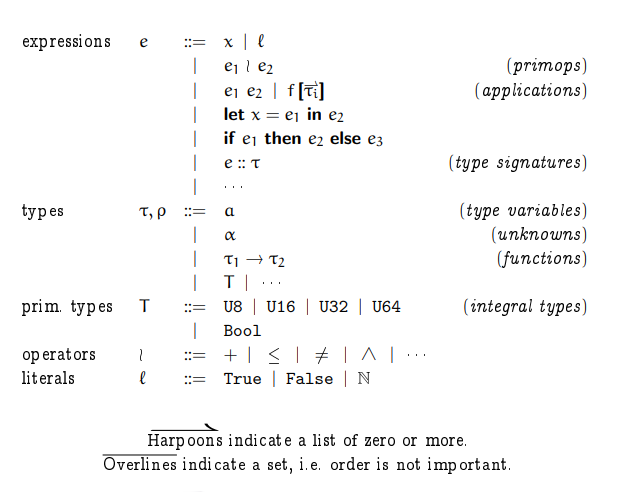
\includegraphics[width=350pt]{content/CogentGrammar.png}
    \caption{The basic syntax for Cogent~\citep{ICFPCogent}}
    \label{fig:cogentGrammar}
\end{figure}

%%% Variant syntax
\begin{figure}
    \centering
    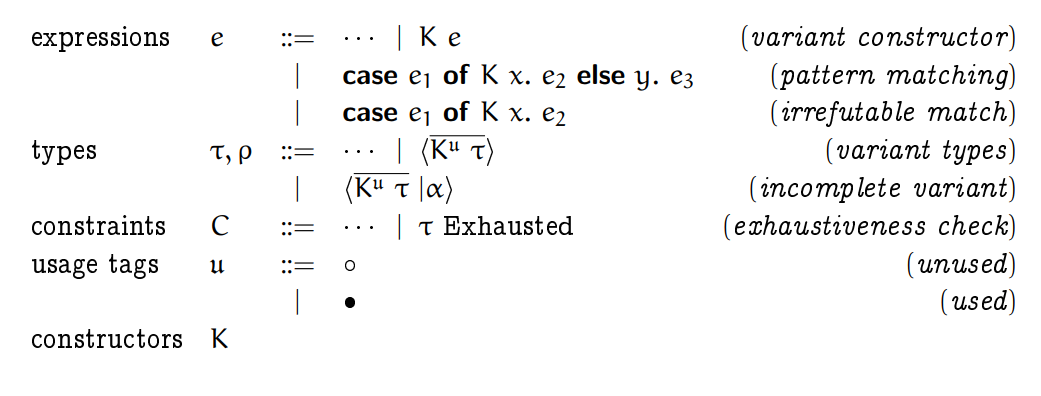
\includegraphics[width=400pt]{content/VariantGrammar.png}
    \caption{The syntax for variant types within Cogent~\citep{ICFPCogent}}
    \label{fig:variantGrammar}
\end{figure}

%%% Record syntax
\begin{figure}
    \centering
    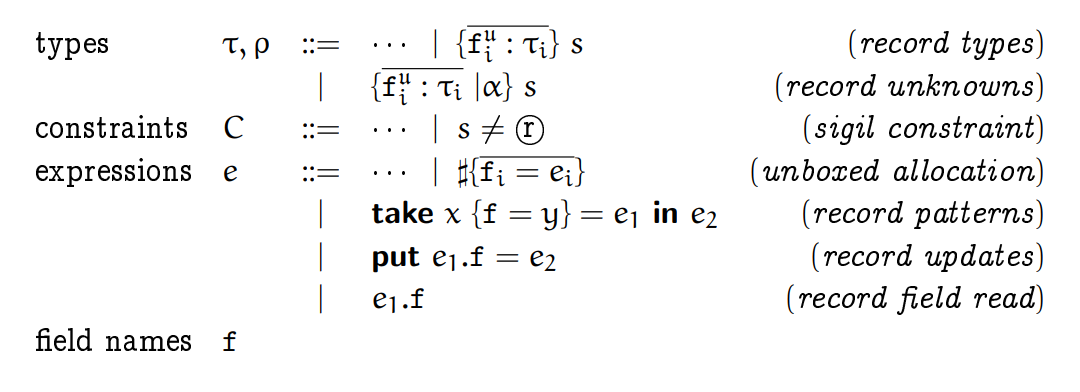
\includegraphics[width=400pt]{content/RecordGrammar.png}
    \caption{The syntax for record types within Cogent~\citep{ICFPCogent}}
    \label{fig:recordGrammar}
\end{figure}



Cogent's uniqueness type system features a variety of basic types as well as the more advanced variants
and records.

\subsection{Primitive Types}

Cogent's primitive datatypes consist of \textbf{Bools}, and the four unsigned integer types \textbf{U8}, 
\textbf{U16}, \textbf{U32} and \textbf{U64}. Integer types can be upcast using the \textbf{upcast}
keyword to convert a smaller integer type into a larger one (e.g. a \textbf{U8} into a \textbf{U32}).
Details of these types can be seen in the syntax for Cogent's basic grammar in figure \ref{fig:cogentGrammar}.

Each of these primitive types are of fixed size, and thus are \textbf{unboxed}, meaning they are stored on the
stack. They are not subject to the use exactly once constraint that uniqueness types enforce.

Cogent also features \textbf{tuples} (product types) through the standard tuple syntax across the ML
family of languages: $(a,b)$, and standard functions, however they are limited to one argument.

\subsection{Variant Types}

Cogent's variant types are inspired from the traditional sum/option types, where a variant type man contain
one of many specified types, the syntax for which is defined in figure \ref{fig:variantGrammar}.

Consider the following example, we can reconstruct \textit{Haskell's} Maybe type using our variants:

\begin{center}
    \textbf{type} \textit{Maybe} a = $\langle$ Nothing () $\vert$ Just a $\rangle$
\end{center}

Or a type to represent a choice of colours:

\begin{center}
    \textbf{type} \textit{RGB} = $\langle$ Red () $\vert$ Green () $\vert$ Blue () $\rangle$
\end{center}

Pattern matching on variants must be \textit{complete}, i.e. you must give a case for every possible constructor
of a variant, a constraint that helps keep functions total.

Variant types work well as a potential constructor for our recursive types. If we were to reference a
recursive parameter inside the variant, we would be able to create a recursive structure similar to Haskell.
However, as variants are \textit{unboxed} (stored on the fixed size stack), we cannot allow for dynamically sized structues
using only variants, so we must look elsewhere for a solution.

\subsection{Record Types}

Cogent's record types are similar to \textit{structs} with names fields. They come in two forms, \textit{boxed}
(stored dynamically on the heap) or \textit{unboxed} (stored statically in the stack), the syntax of both is
as in figure \ref{fig:recordGrammar}.

For example, consider a record to bundle together user information:

\begin{center}
    \begin{tabular}{l}
    \textbf{type} \textit{User} = \{ \\
                    \hspace{1.5em} name: \textit{String},\\
                    \hspace{1.5em} age: \textit{U32}, \\
                    \hspace{1.5em} favouriteColour: \textit{RGB}\\
                    \} \\
    \end{tabular}
\end{center}

Records allow for us to create dynamically sized objects, as we can used boxed records to chain together a
combination of records on the heap. With the aid of variant types, records can allow us to construct our recursive 
types with a recursive paramater included to reference the type overall type, using variants to give the 
differing construction cases for the type.

\section{Termination And Recursive Types}

Proving total correctness about the programs we write is a very desirable result,
as computation performed by a program is useless if the program never returns the
result of the computation we desire.
In a systems context, termination is especially desirable as an infinitely looping component of a
system could cause it to hang, ruining the experience for end users of the system.

Our focus for reasoning about termination falls on considering the use of Isabelle to verify our 
embedding as well as facilitating the ease of this process at the type level within Cogent. 

\subsection{Proving Termination in Isabelle}


The official Isabelle tutorial\citep{IsabelleTutorial} describes 3 methods of creating functions using the keywords 
\textbf{primrec}, \textbf{fun} and \textbf{function}. The first, \textbf{primrec}, allows one to create a 
\textit{primitive recursive} function --- one that returns a constant or removes a data type constructor from one
of the arguments to the function in its body, `decreasing' in size every time. These functions are \textit{total}
and always terminate, removing the need of a termination proof (which is required for all functions within Isabelle,
unless they are defined to be partial, however this is undesirable).
Primitive recursive functions however are limited in their expressiveness and are a subset of all computable
functions, so we cannot rely on them for the general case.

In his tutorial\citep{KraussIsabelle}, Alexander Krauss discusses the details of the latter two of the 3 methods
of creating functions in Isabelle. The \textbf{fun} keyword instructs Isabelle to try and solve all necessary
termination proof obligations, rejecting the definition if it fails (either because the definition does not 
terminate or because Isabelle cannot figure out how to prove it does). In contrast to \textbf{fun}, \textbf{function}
requires that the termination proofs be solved manually by whoever is writing the proof.

\amos{Worth comparing the `gas' or `clock' approach as well, as used by CakeML (see CakeML: A Verified Implementation of ML, POPL 2014).
There, the embedding of the program has an extra parameter which is a natural number describing how much time the program has to compute a result.
At each recursive step, the clock is decremented, and if it reaches zero the program runs out of time and throws an exception.
This lets you embed arbitrary programs as primitive recursion on a nat.
You have to prove termination separately, but you can reason about the program assuming termination (assume that there exists a large enough clock that the program will return a valid value).}

\todo{Relate to proposal}

\subsection{Strictly Positive Types}

Adding recursive types to a type system allows for expressions that are potentially infinitely recursive,
as discussed by Wadler~\cite{RecursiveTypesForFree}, who explains the potential for recursive expressions
to cause non-termination through polymorphic lambda calculus. In his paper, he discusses how this
quality can be qualified with positive and negative data types.

Suppose a data type in its general form $T$ and its data constructors $C_{1..n}$, each with a number of arguments 
$\tau_{i1}..\tau_{ik}$:

\begin{center}
    \begin{tabular}{l}
        $T = C_1\; \tau_{11} \; \tau_{12} \; \dots$ \\
        $\hspace{1.5em} \vert\; C_2\; \tau_{21} \; \tau_{22} \; \dots$ \\
        $\hspace{1.5em} \vert\; \dots$ \\
    \end{tabular} 
\end{center}

\theoremstyle{definition}
\begin{definition}
    A data type $T$ is said to be in a \textit{negative position} if $T$ appears nested as an argument
    to a function an odd amount of times inside any $\tau_{ij}$, and said to be in a \textit{positive position}
    if $T$ appears nested as an argument to a function an even amount of times inside $\tau_{ij}$.
\end{definition}

\theoremstyle{definition}
\begin{definition}
    A data type $T$ is a \textit{negative} data type if it appears in a negative position 
    in one of its constructors.
\end{definition}

\theoremstyle{definition}
\begin{definition}
    A data type $T$ is a \textit{positive} data type if only appears nested in a positive position
    in all of its constructors.
\end{definition}

In simpler terms, if $T$ appears to the left of a function arrow an odd amount of times, it is negative and if
to the left an even amount of times then it is positive.

For example:

\begin{center}
    \begin{tabular}{l}
        $E = C\; (\underline{E} \rightarrow E)$ \\
        $K = D\; (\underline{(\underline{K} \rightarrow_1 Int)} \rightarrow_2 K)$
    \end{tabular} 
\end{center}

Here, the data type $E$ is negative as it appears in a negative position (denoted here by an underline)
to a function in the first argument of $C$.
$K$ however is positive as it appears only ever in a positive position as it is nested as an argument
in function 1 ($\rightarrow_1$) and again in function 2 ($\rightarrow_2$) for a total of two times.

Allowing for negative types in our system allows for data structures that are infinitely recursive,
which if iterated over would potentially cause non-termination. Consider
the following example in \textit{Haskell}:

\lstinputlisting[language=haskell]{content/NegativeType.hs}

By our definition, we can see that our type \textit{Bad} is a \textit{negative} type and using it we were able
to construct the infinitely recursive expression, \textbf{g (A g)}.
This is not an issue in Haskell due to its lazy evaluation,
however as Cogent is not lazily evaluated these expressions would be undesirable in
our language as iterating over them potentially results in non-termination, and in this
situation hang when \textit{infiniteExpression} is constructed.
Although this example was constructed maliciously, situations may arise where
programmers may accidentally construct such an expression, so we must seek a way to
eliminate them from our language.

Many theorem provers and dependently typed languages make use of \textit{strictly positive} types, which
prohibit the construction of infinitely recursive data structures that under a dependant type system
both negative and simple positive types allow.
\textit{Agda}\citep{AgdaStrictlyPositive}, \textit{Coq}\citep{CoqStrictlyPositive} and even
Isabelle\citep{IsabelleStrictlyPositive} features this exact constraint, as allowing for negative
or normal positive types introduce logical inconsistencies which can be used to prove false statements,
something that is unacceptable for a theorem prover.

The definition of strictly positive is discussed by Coquand and Paulin~\cite{CoquandTypes}, and is as follows:

\theoremstyle{definition}
\begin{definition}
    \label{def:sp}
    Given a data type $T$ and its constructors $C_{1..n}$, for every argument $\tau_{ij}$
    of any data constructor $C_i$ wher $\tau_{ij}$ is a function, $T$ is said to be \textit{strictly positive} if 
    $T$ does not occur as an argument to any $\tau_{ij}$:

    \begin{center}
        $\forall\; \tau_{ij}.\;
        (\tau_{ij} = \phi_{1} \rightarrow \dots \rightarrow \phi_{k})
        \implies T \notin \phi_{1..k-1}$
    \end{center}
\end{definition}

Strictly positive types can also be defined as types where $T$ appears in a negative or positive 
position exactly zero times (i.e. it does not appear to the left of any arrow).

In their paper, Conquand and Paulin further discuss the ability to produce an \textit{eliminator} or a
\textit{fold} from any strictly positive type, which corresponds to an induction principle on the type.

Consider a type for natural numbers with two constructors for zero and successor:

\begin{center}
    \begin{tabular}{l}
        $Nat = \textsc{Z}\; \vert\; \textsc{S}\; Nat$ \\
    \end{tabular} 
\end{center}

We can see $Nat$ is a strictly positive type and the induction principle it produces
for any predicate over natural numbers, $P$, is:

\[
    \infer{
        \forall(N : Nat).\;\; P(N)
    }{
        P(Z) \quad & \forall (X : Nat).\; P(X) \implies P(S\; X)
    }
\]

Where in order to prove our predicate $P$, we prove it for each case of how our type $T$ could have been
constructed, which each constructor for our our type supplies.
That is, to prove any predicate $P$ inductively over nats ($\forall(N : Nat).\; P(N)$)
we prove it for the base (zero) case $P(Z)$ and then assuming the predicate holds
for a natural number $X$, we prove it for its successor case $S\; X$: $P(X) \implies P(S\; X)$.

The interactive theorem prover Isabelle generates the same induction principle for any type created in
Isabelle. We can get the same induction principle over natural numbers by redefining our $Nat$
type in Isabelle, as in figure \ref{fig:IsabelleNatInduct}.

\begin{center}
    \begin{figure}
        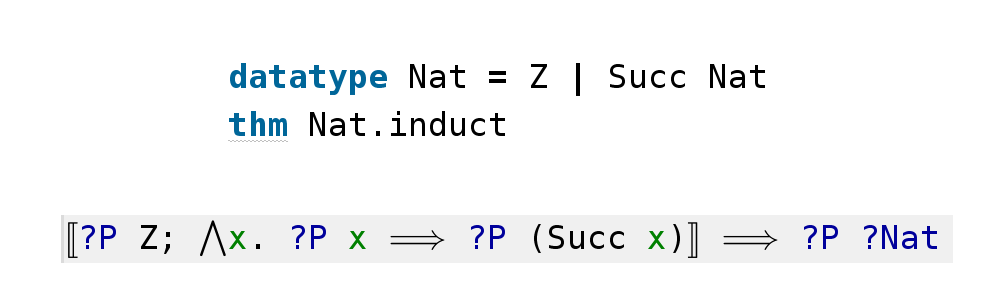
\includegraphics[width=\linewidth]{content/isabelleNatInduct.png}
        \caption{A type for natural numbers defined in Isabelle, and the generated 
        induction principle associated with the type.}
        \label{fig:IsabelleNatInduct}
    \end{figure}
\end{center}

\FloatBarrier

Considering our Cogent embedding will be within Isabelle, if we can embed our native
Cogent types into an Isabelle type then we gain Isabelle's automatically generated
induction principle over our Cogent types, allowing for much 
simpler reasoning about our Isabelle embedding.

\section{Linear And Uniqueness Types}

Linear types are a kind of substructural type system as discussed by\newline David Walker~\citep{Substructural}.
Many standard programming languages such as \textit{C}, \textit{Java} and \textit{Haskell} feature
three standard structural typing rules, described in figure \ref{def:structural}.

\begin{figure}
    \centering
    $$
        \infer[Exchange]{
            \Gamma_1\Gamma_2 \vdash e : \tau
        }{
            \Gamma_2\Gamma_1 \vdash e : \tau
        }\quad
        \infer[Weakening]{
            \Gamma_1\Gamma_2 \vdash e : \tau
        }{
            \Gamma_1 \vdash e : \tau
        }\quad
        \infer[Contraction]{
            \Gamma_1\Gamma_2 \vdash e : \tau
        }{
            \Gamma_1\Gamma_1\Gamma_2 \vdash e : \tau
        }
    $$
    \caption{Structural typing rules}
    \label{def:structural}
\end{figure}

\textit{Exchange} is the rule that states that the order in which we add variables in an environment
is irrelevant. A conclusion of this is that if a term $e$ typechecks under environment $\Gamma$,
then any permutation of $\Gamma$ will also typecheck $e$.

\textit{Weakening} states that if a term $e$ typechecks under the assumptions
in $\Gamma_1$, then $e$ will also typecheck if extra assumptions are added to the environment.

\textit{Contraction} states that if we can typecheck a term $e$ using two identical
assumptions, then we are able to check $e$ with just one of those two assumptions.

Substructural type systems however control access to information within the program by limiting which
of the structural typing rules are allowed under certain contexts. Linear types ban the use of the
contraction and weakening rules, which has the consequence that all linear variables must be used 
at least once (by lack of weakening) and at most once (by lack of contraction), hence exactly one time.

One powerful benefit that linear types allow is \textit{static allocation} of objects, which Cogent
features. Predicting when an object in a program will be last used (and after deallocated)
is undecidable as it is a nontrivial semantic property by Rice's Theorem~\citep{Sipser},
however in a linear type system we know exactly when an object will be freed,
which is exactly after its first use by the use once rule. The result is a langauge that does
not require a garbage collector, and doesn't require users to explicitly declare memory allocation,
as this can now be determined statically.

Wadler~\cite{LinearTypesChangeTheWorld} also describes the performance benefits of destructive updates
that linear types grant. As we have a guarantee that no other part of a program is referencing a particular
object (variables must be used exactly once), when performing an operation on an object, the resultant
object can be our old object with the result of our operation performed in place (i.e. destructively
mutated).

Consider the following program in Java:

\lstinputlisting[language=Java,basicstyle=\small]{content/destructive.java}

In this example we attempt to double a copy of a list of numbers in place by use of the \verb|doubleNumbers|
function on \verb|copyOfNumbers|, however by updating it in place has changed the original variable outside
the function \verb|oldNumbers|. If a programmer mistakenly uses \verb|oldNumbers| again without realising that
\verb|doubleNumbers| has mutated it instead of a copy of it, it would most likely cause an error. In 
Java this kind of destructive update cannot be done safely whilst \verb|oldNumbers| still exists, and we
must resort to copying.

Linear types prevent this kind of mistake, as the duplicate reference that
\verb|oldNumbers| and \verb|copyOfNumbers| share would be eliminated once \verb|oldNumbers| is used once,
which in turn allows for a desctructive update on \verb|oldNumbers| to take place with the result stored in
copyOfNumbers.

While Cogent already features these guarantees, \todo{Difference between uniqueness and linear, link back to
Cogent}